\chapter{Sistema Quadrirotore}
Il capitolo è incentrato sulla descrizione del modello matematico del sistema quadricottero con le relative dinamiche, leggi di guida e leggi di controllo possibili da implementare.
\section{Modello matematico}
Il principio di funzionamento del quadrirotore è relativamente semplice nel suo complesso. Come accennato in precedenza la gestione dell'assetto è ottenuta attraverso l'azionamento differenziale dei rotori, montati su di una struttura rigida \cite{modelquad}.
Nel seguente elenco di manovre di base, viene preso come riferimento la Figura (\ref{fig:modello_quad}).
\begin{figure}
	\centering
	\begin{subfigure}{0.45\textwidth}
		\centering
		\includegraphics[width=1\textwidth]{SistemaQuadrirotore/Figure/drone_alto}
		\caption{Numerazione rotori}
		\label{fig:modello_quad}
	\end{subfigure}
	\hfill
	\begin{subfigure}{0.45\textwidth}
		\centering
		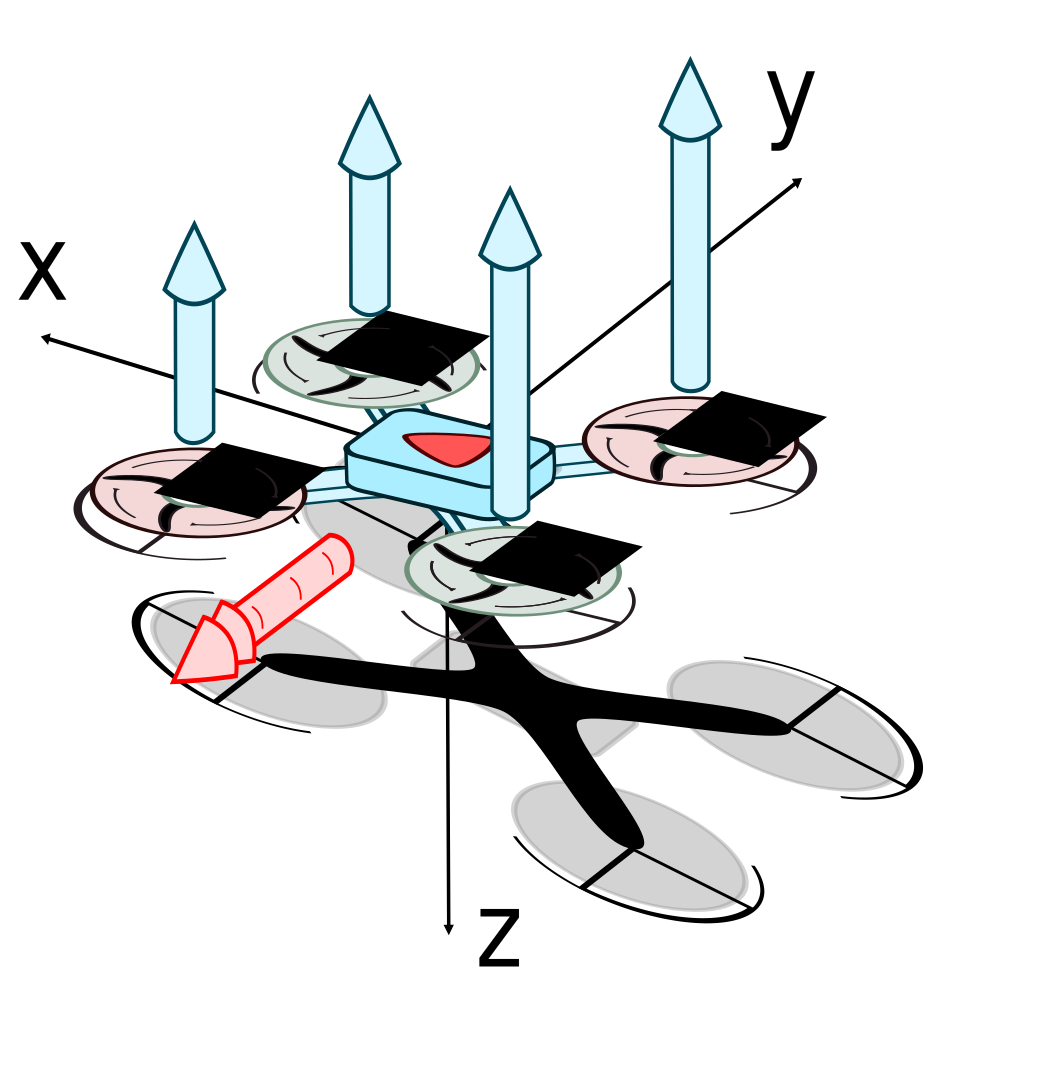
\includegraphics[width=1\textwidth]{SistemaQuadrirotore/Figure/drone_pitch}
		\caption{Variare l'angolo di beccheggio}
		\label{fig:modello_quad_pitch}
	\end{subfigure}
	\\
	\begin{subfigure}{0.45\textwidth}
		\centering
		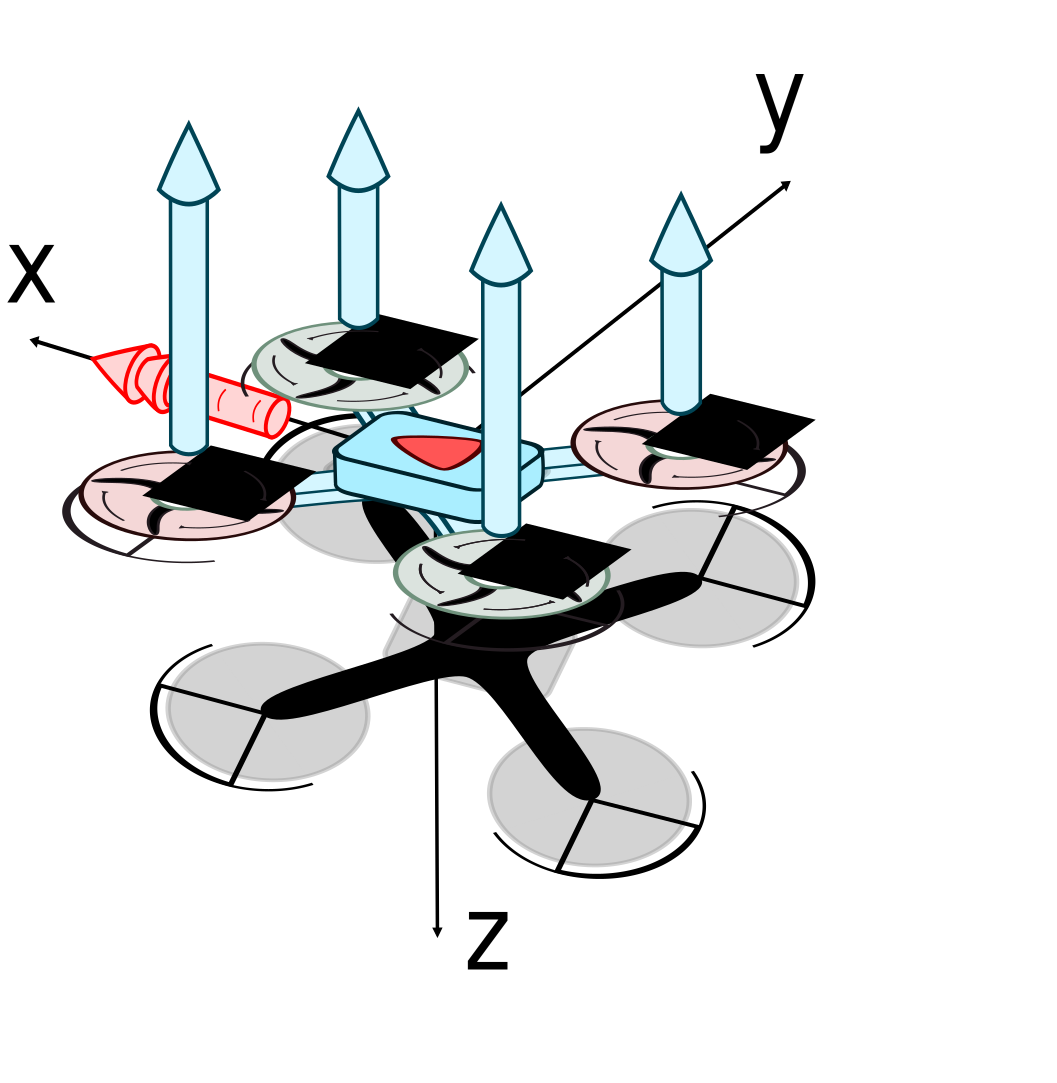
\includegraphics[width=1\textwidth]{SistemaQuadrirotore/Figure/drone_roll}
		\caption{Variare l'angolo di rollio}
		\label{fig:modello_quad_roll}
	\end{subfigure}
	\hfill
	\begin{subfigure}{0.45\textwidth}
		\centering
		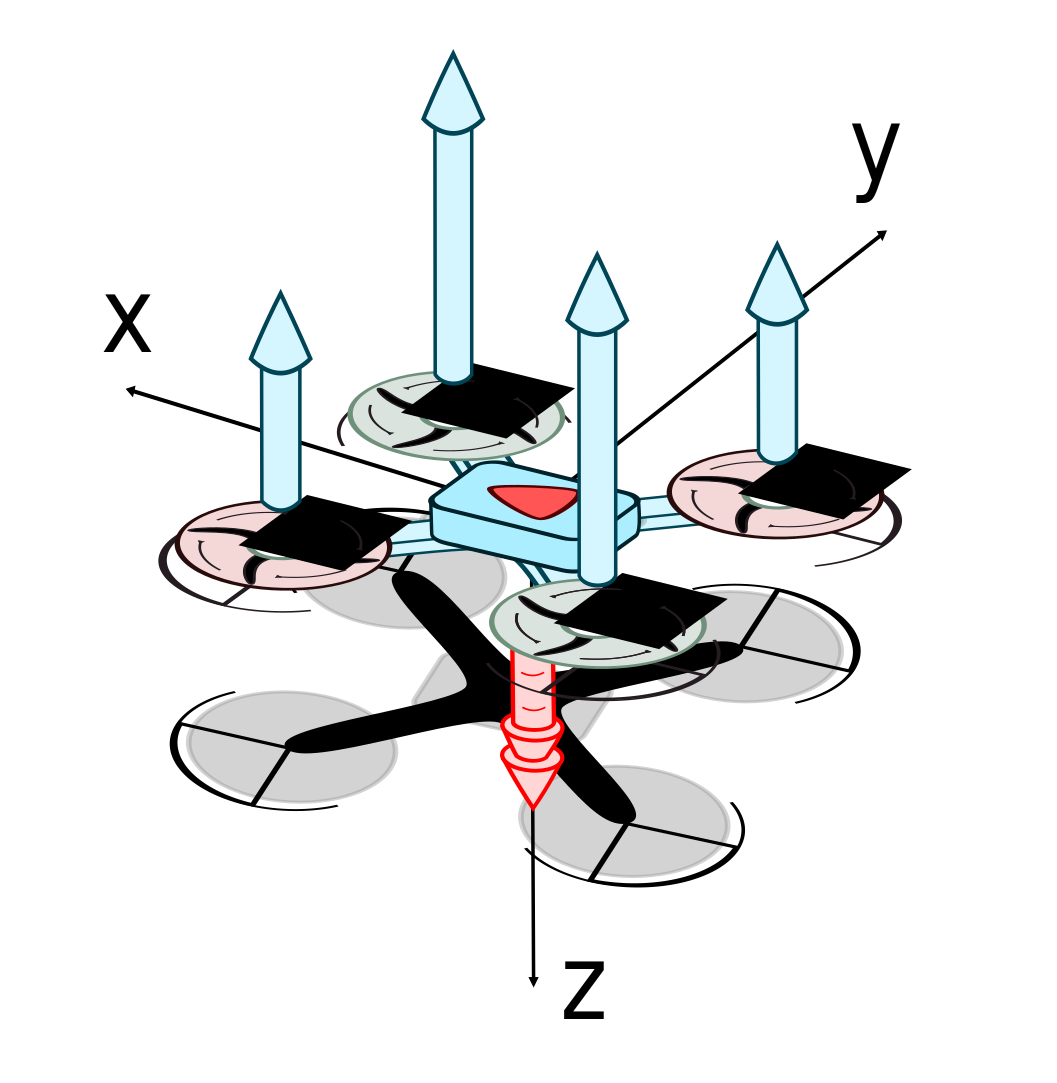
\includegraphics[width=1\textwidth]{SistemaQuadrirotore/Figure/drone_yaw}
		\caption{Variare l'angolo di imbardata}
		\label{fig:modello_quad_yaw}
	\end{subfigure}
	\caption{Schemi semplificati dell'azionamento del quadrirotore}
\end{figure}
\begin{itemize}
	\item \textbf{Comando di beccheggio:} Una variazione di beccheggio positiva lungo l'asse y del corpo del drone avviene comandando una maggiore velocità ai rotori 2 e 3 rispetto ai 1 e 4, come mostrato nella Figura (\ref{fig:modello_quad_pitch})
	\item \textbf{Comando di rollio:} Una variazione di variazione dell'angolo di rollio positiva si ottiene modificando la velocità di azionamento dei rotori in modo simmetrico rispetto all'asse y del drone. Come mostra la Figura (\ref{fig:modello_quad_roll}) una variazione positiva si ottiene facendo ruotare i rotori 1 e 3 più lentamente dei rotori 2 e 4.
	\item \textbf{Comando di imbardata:} Questo comando è il meno efficace nel quadricottero in quando viene implementato attraverso un effetto secondario. Come si vede nella Figura (\ref{fig:modello_quad_yaw}), la rotazione dei rotori viene, mantendendo la portanza totale costante, distribuita in modo differente tra le pale che ruotano in modo orario e antiorario. Il comando di variazione positivo dell'angolo di imbardata si ottiene facendo ruotare più rapidamente i rotori 1 e 2 rispetto a 3 e 4.
	\item \textbf{Comando di spinta complessiva : } La variazione di quota avviene grazie a questo tipo di comando. Aumentando o diminuendo in modo identico la velocità di rotazione dei rotori è possibile equilibrare il peso, contrastato dalla portanza da essi generata. Una portanza maggiore si traduce in una accelerazione verso l'alto, viceversa si traduce in una diminuzione di quota.
\end{itemize}
Grazie a questo funzionamento e l'utilizzo di un mixer, che ha lo scopo di miscelare i quattro tipi di azionamento visti, si può governare il velivolo modificandone la posizione nello spazio \cite{DesTestCarm}.
\subsubsection{Relazioni matematiche}
Verranno esplicitate alcune formule utili per la modellazione iniziale del problema del quadrirotore come riportato in bibliografia, \cite{DesTestCarm}, \cite{baseTesi}. Le ipotesi di partenza della trattazione prevedono di considerare come corpi rigidi tutti i componenti, di supporre trascurabile le forze aerodinamiche diverse dalla spinta principale del rotore. Inoltre viene considerato un sistema di riferimento terrestre come fosse inerziale, conosciuto come modello di terra piatta.

Utilizzando i sistemi di riferimento del corpo del drone e del riferimento terreste come in Figura (\ref{fig:riferimenti}), si definisce la matrice di rotazione $R$ espressa dalla relazione (\ref{eq:SistemaQuadrirotore_R}). In questo sistema si impone che l'asse $x$ del corpo sia diretto verso il muso del drone e l'asse $y$ verso destra, in modo che l'asse $z$ sia diretto verso il basso, mentre l'asse $x_e$ risulta essere diretto verso nord, l'asse $y_e$ verso est e di conseguenza l'asse $z_e$ verso il centro della terra. 
Attraverso il sistema di equazioni, espresso in forma matriciale (\ref{eq:SistemaQuadrirotore_ratei}), si ricavano i ratei degli angoli di assetto partendo dalle accelerazioni angolari, utilizzando per  comodità le seguenti semplificazioni di scrittura, $ c(\cdot)=\cos(\cdot)\ ,\  s(\cdot) = \sin(\cdot) $.
\begin{equation}
R=
	\begin{pmatrix}
	c(\psi)c(\theta)-s(\phi)s(\psi)s(\theta) & -c(\phi)s(\psi) & c(\psi)s(\theta)+c(\theta)s(\theta)s(\psi) \\ 
	c(\theta) s(\psi)+c(\psi)s(\phi)s(\theta) & c(\phi)c(\psi) & s(\psi)s(\theta)-c(\psi)c(\theta)s(\phi) \\ 
	-c(\phi)s(\theta)	& s(\phi) & c(\phi)c(\theta)
	\end{pmatrix}
	\label{eq:SistemaQuadrirotore_R}
\end{equation}
\begin{equation}
	\begin{Bmatrix}
		\dot{\phi}\\
		\dot{\theta}\\
		\dot{\psi}
		\end{Bmatrix}=
	\begin{pmatrix}
		1 & \sin(\phi)\tan(\theta) & \cos(\phi)\tan(\theta) \\ 
		0 & \cos(\phi) & -\sin(\phi) \\ 
		0 & \frac{\sin(\phi)}{\cos(\theta)} & \frac{\cos(\phi)}{\cos(\theta)}
	\end{pmatrix}
	\begin{Bmatrix}
		p\\
		q\\
		r
	\end{Bmatrix}
	\label{eq:SistemaQuadrirotore_ratei}
\end{equation}

\begin{figure}
	\centering
	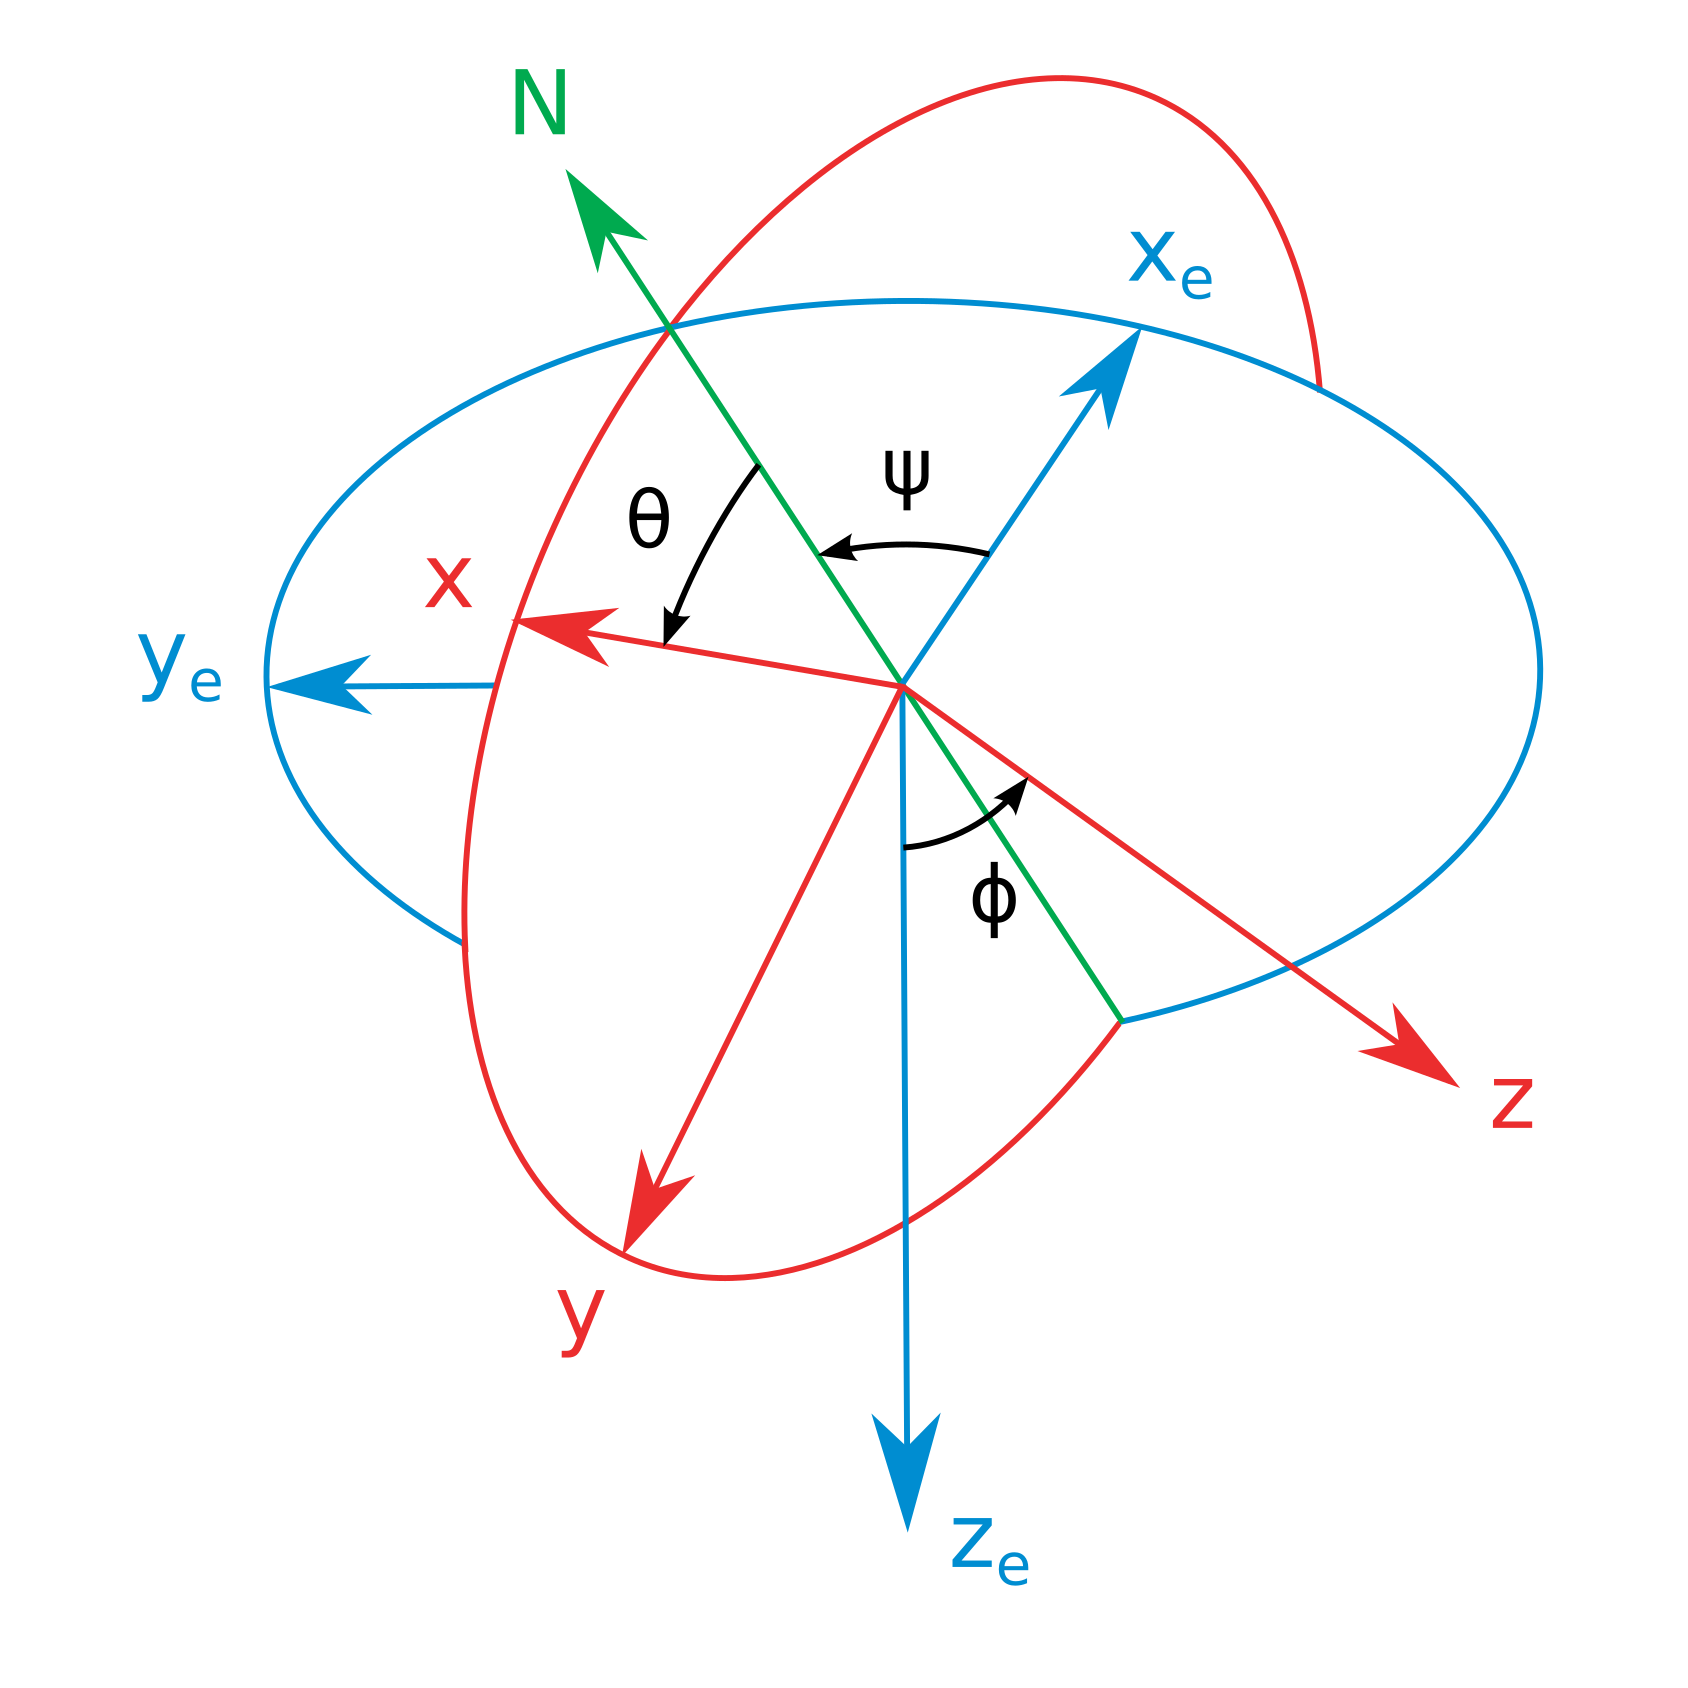
\includegraphics[width=0.33\textwidth]{SistemaQuadrirotore/Figure/eulerangles.png}
	\caption{Rotazione tra sistemi di riferimento NED e corpo \cite{eulero}}
	\label{fig:riferimenti}
\end{figure}

Risulta utile presentare anche la rappresentazione di rotazioni nello spazio attraverso l'uso di quaternioni, molto utilizzata in applicazioni robotiche grazie alla possibilità di superare le limitazioni dovute alle singolarità presenti nella rappresentazione euleriana.
Si definisce quindi un quaternione:
\[ 
	\mathfrak{q} = q_0 + q_1 \mathbf{i} + q_2 \mathbf{j} + q_3 \mathbf{k}
\]
Per comodità si utilizzeranno le scritture nelle forme :
\[ 
	\mathfrak{q} = \begin{Bmatrix}
		q_0\\
		\mathbf{q}
	\end{Bmatrix} \ , \ \mathbf{q} = \begin{Bmatrix}
		q_1\\
		q_2\\
		q_3
	\end{Bmatrix}
\]
Nella definizione del quaternione $\mathbf{i}$,$\mathbf{j}$ e $\mathbf{k}$ sono l'equivalente di numeri complessi che godono tra di loro della proprietà di ortogonalità, mentre $q_0$, $q_1$, $q_2$ e $q_3$ sono numeri reali. Utilizzando la definizione del prodotto di Hamilton, Eq.  (\ref{eq:SistemaQuadrirotore_hamilton}), si può determinare il quaternione rappresentante l'errore da minimizzare nella fase di controllo, nella Eq. (\ref{eq:SistemaQuadrirotore_errore}), dove $\mathfrak{q}_{est}$ è la misurazione e $ \mathfrak{q}_{ref}$ e il riferimento.
\begin{equation}\label{eq:SistemaQuadrirotore_hamilton}
	\mathfrak{q} \otimes \mathfrak{p} = q_0 p_0 - \mathbf{q} \cdot \mathbf{p} + q_0 \mathbf{p} + p_0 \mathbf{q} + \mathbf{q} \times \mathbf{p}
\end{equation}
\begin{equation}\label{eq:SistemaQuadrirotore_errore}
	\mathfrak{q}_{err} = \mathfrak{q}_{est}^{-1} \otimes \mathfrak{q}_{ref}
\end{equation}
La derivata del quaternione nel tempo è esprimibile attraverso la relazione (\ref{eq:SistemaQuadrirotore_quaternionederivato}), dove $p$, $q$ ed $r$ sono i ratei di rotazione rispetto agli assi $x$, $y$ e $z$,rispettivamente.
\begin{equation}\label{eq:SistemaQuadrirotore_quaternionederivato}
\mathfrak{\dot{q}} = \frac{1}{2} \mathbf{\Omega} \mathfrak{q} =
	\begin{pmatrix}
		0 & -p & -q & -r \\
		p &  0 &  r & -q \\
		q &  r &  0 &  p \\
		r &  q & -p &  0 
	\end{pmatrix}
	\begin{Bmatrix}
		q_0 \\
		\mathbf{q}
	\end{Bmatrix}
\end{equation}
Utilizzando le formule (\ref{eq:SistemaQuadrirotore_Forze}) e (\ref{eq:SistemaQuadrirotore_momenti}) si determinano relativamente le forze e i momenti applicati. Manipolando le relazioni precedenti si possono ottenere le accelerazioni e le accelerazioni angolari, Eq. (\ref{eq:SistemaQuadrirotore_acc}) e (\ref{eq:SistemaQuadrirotore_accang}), rispettivamente. Per esplicitare le accelerazioni angolari è necessario considerare la formula (\ref{eq:SistemaQuadrirotore_momento_qdm}) che esprime il momento della quantità di moto.
\begin{equation}\label{eq:SistemaQuadrirotore_Forze}
	\mathbf{F} + \mathbf{R} m \mathbf{g} = m \left[\frac{d \mathbf{v}}{d t} + \boldsymbol{\omega}\times \mathbf{v}\right]
\end{equation}

\begin{equation}\label{eq:SistemaQuadrirotore_acc}
	\frac{\mathbf{F}}{m} + \mathbf{R} \mathbf{g} = \mathbf{\dot{v}} + \boldsymbol{\omega} \times \mathbf{v}
\end{equation}

\begin{equation}\label{eq:SistemaQuadrirotore_momenti}
	\boldsymbol{\tau} = \frac{d \mathbf{H}}{d t } + \boldsymbol{\omega} \times \mathbf{H}
\end{equation}

\begin{equation}\label{eq:SistemaQuadrirotore_momento_qdm}
	\mathbf{H} = \mathbf{J} \boldsymbol{\omega} =
	\begin{pmatrix}
		J_x & J_{xy} & J_{xz} \\
		-J_{xy} & J_y & -J_{yz} \\
		-J_{xz} & -J_{yz} & -J_z 
	\end{pmatrix}
	\begin{Bmatrix}
		p\\
		q\\
		r
	\end{Bmatrix}
\end{equation}

\begin{equation}\label{eq:SistemaQuadrirotore_accang}
	\boldsymbol{\dot{\omega}} = - \mathbf{J^{-1}}\left(\boldsymbol{\omega}\times\left(\mathbf{J}\boldsymbol{\omega}\right)\right) + \mathbf{J^{-1}}\boldsymbol{\tau}
\end{equation}

Si definiscono il vettore di stato e di comando come segue:
\[ 
	\mathbf{x} = \begin{Bmatrix}
		x \\ y \\ z \\ \phi \\ \theta \\ \psi \\ u \\ v \\ w \\ p \\ q \\ r
	\end{Bmatrix}, \  \mathbf{u} = \begin{Bmatrix}
	F_x \\ F_y \\ F_z \\ \tau_x \\ \tau_y \\ \tau_z
	\end{Bmatrix}
\]
Si definiscono inoltre le costanti : 
\[ 
	\begin{matrix}
	c_1 = \frac{J_{xz} (J_x -J_y + J_z)}{J_x J_y- J_{xz}^2} , & c_2 = \frac{J_{xz} (J_x -J_y +J_z)}{J_x J_y-J_{xz}^2}, &c_3 \frac{J_z}{J_x J_y - J_{xz}^2}, \\
	c_4 = \frac{J_{xz}}{J_x J_y -J_{xz}^2} ,& c_5 = \frac{J_z - J x}{J_y},& c_6 = \frac{J_{xz}}{J_y}, \\
	c_7 = \frac{1}{J_y} ,& c_8 = \frac{J_{xz}^2 + J_x (J_x - J_y)}{J_x J_y - J_{xz}^2},& c_9 =  \frac{J_x}{J_x J_y -J_{xz}^2}
	\end{matrix}
\]

Con le formule precedenti, si riformulano le equazioni differenziali ottenendo la scrittura nello spazio degli stati, Eq. (\ref{eq:SistemaQuadrirotore_statespace}).
\begin{equation}\label{eq:SistemaQuadrirotore_statespace}
\mathbf{\dot{x}} = \mathbf{f(x)} + \mathbf{g} \cdot \mathbf{u},
\end{equation}
Dove
\[
	\mathbf{f(x)} = \begin{Bmatrix}
		\mathbf{R} \begin{Bmatrix}
			u \\ v \\ w
		\end{Bmatrix} \\
		p + (q\sin(\phi)+r\cos(\phi))\tan(\theta) \\
		q\cos(\phi) - r\sin(\phi) \\
		\frac{q\sin(\phi) - r\cos(\phi)}{\cos(\theta)}\\
		rv-qw-g\sin(\theta)\\
		-ru + pw p g \sin(\phi)\cos(\theta)\\
		qu - pv + g \cos(\phi)\cos(\theta)\\
		q (c_1 r + c_2 p)\\
		c_5 pr - (p^2-r^2) c_6 \\
		q(c_8 p - c_2 r)
	\end{Bmatrix}, \ \mathbf{g} =
	\begin{pmatrix}
		0 & \cdots & \cdots & \cdots & \cdots & 0 \\
		0 & \ddots & & & & \vdots \\
		0 & & \ddots & & & \vdots \\
		0 & & & \ddots & & \vdots \\
		0 & & & & \ddots & \vdots \\
		0 & \cdots & \cdots & \cdots & \cdots & 0 \\
		\frac{1}{m} & 0 & \cdots & \cdots & \cdots & 0 \\
		0 & \frac{1}{m} & 0 & \cdots & \cdots & 0 \\
		0 & 0 & \frac{1}{m} & 0 & \cdots & 0 \\
		0 & \cdots & 0 & c_3 & 0 & c_4 \\
		0 & \ddots & \vdots & 0 & c_7 & 0 \\
		0 & \cdots & 0 & c_4 & 0 & c_9 \\
	\end{pmatrix}
\]

Il modello matematico rappresentativo del comportamento del quadricottero è ottenibile integrando le equazioni sopra riportate.

Nel precedente studio il contributo della spinta introdotta dalla presenza dei rotori era stata ricavata sperimentalmente su di un banco di prova \cite{DesTestCarm}. In questa tesi verranno utilizzate le stesse leggi quadratiche ricavate e rappresentate in Figura (\ref{fig:pwmTM}). Questi sono necessari per valutare il vettore di comando, presentato dalla formula (\ref{eq:SistemaQuadrirotore_vettorecomando}), dove $l$ rappresenta il braccio del rotore rispetto al centro di massa.

\begin{equation}\label{eq:SistemaQuadrirotore_vettorecomando}
	\mathbf{u}(\nu_1,\nu_2,\nu_3,\nu_4) = 
	\begin{Bmatrix}
		F_x \\ F_y \\ F_z \\ \tau_x \\ \tau_y \\ \tau_z
	\end{Bmatrix}
	=\begin{Bmatrix}
		0 \\ 0 \\
		-\left[F(\nu_1)+F(\nu_2)+F(\nu_3)+F(\nu_4)\right] \\
		\left[F(\nu_4)+F(\nu_2)-F(\nu_1)-F(\nu_3)\right ] l \\
		\left[F(\nu_2)+F(\nu_3)-F(\nu_1)-F(\nu_4)\right] l \\
		\tau(\nu_1)+\tau(\nu_2)-\tau(\nu_3)-\tau(\nu_4)
	\end{Bmatrix}
\end{equation} 
\begin{figure}
	\centering
	\begin{subfigure}{0.45\textwidth}
		\centering
		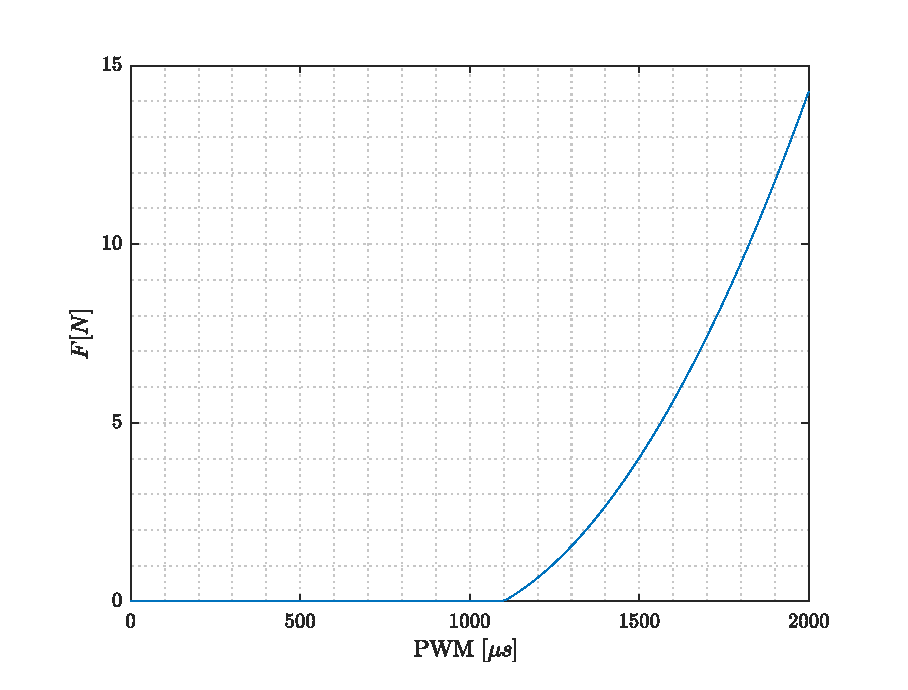
\includegraphics[width=1\textwidth]{SistemaQuadrirotore/Figure/ForzaPWM}
		\caption{Spinta generata in funzione del segnale PWM}
	\end{subfigure}
	\hfill
	\begin{subfigure}{0.45\textwidth}
		\centering
		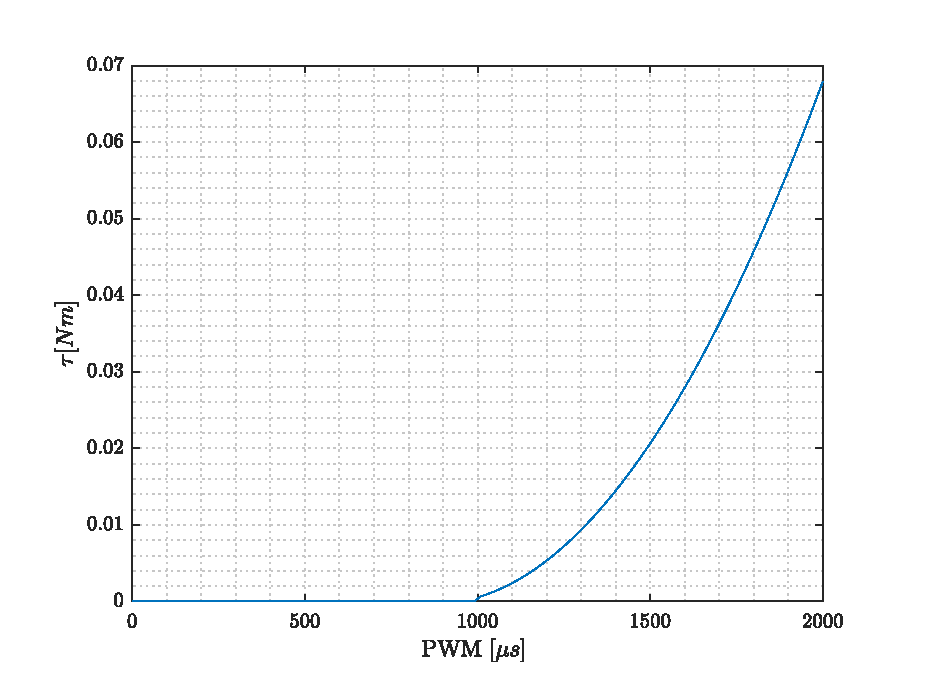
\includegraphics[width=1\textwidth]{SistemaQuadrirotore/Figure/MomentoPWM}
		\caption{Momento generato in funzione del segnale PWM}
	\end{subfigure}
	\caption{Fitting quadratico delle leggi riguardanti il quadrirotore}
	\label{fig:pwmTM}
\end{figure}
 
L'implementazione in Gazebo verrà trattata in dettaglio nel capitolo \ref{section:gazebo}, nella quale verrà descritta anche la parte relativa all'implementazione del disturbo presente nelle misurazioni dei sensori.